\documentclass[acmtog]{acmart}
\usepackage{graphicx}
\usepackage{subfigure}
\usepackage{natbib}

% Title portion
\title{Terrain Modificaiton with fluid simulation using doubly-coupled PCISPH} 
\author{Jiwei Wang \quad Chenghua Yang \quad Yihang Zhu}

% Document starts
\begin{document}
\maketitle

\vspace*{2 ex}


\section{Introduction}
% Present background and related work of the algorithms required in this assignment. Summarize what you have done in this assignment.
In this project, we make an attempt to realize erosion phenomenon applyed on the terrain modification, 
especially on the mountain peak formation in the plate movement. Detailedly, we use PCISPH to simulate fluid behavior.
We utilize marching cube technique to generate mesh by passing volume data. The coupling, including single-sided solid coupling and double coupling,
is implemented to simulate the fluid behavior and terrain change in the erosion process.

\section{Implementation Details}
% Consisely describe the working flow of algorithms. Elaborate on mathematical model and equations of each algorithm. Write down problems you met in the assignment and how you solve them.
\subsection{PCISPH Fluid Simulation}
PCISPH, known as Predictive–Corrective Incompressible SPH, is an incompressible fluid simulation method based on SPH model. 
This method first finds neighbours for each particles and initialize pressure and pressure force accelaration to 0, as well as calculating the force accelaration including gravity and viscosity accelaration.
Then for a given interation number, we repeatedly perform prediction, correction and pressure accelaration compution. \\
In detail, in each iteration, we first predict the velocity and position of each particle at time $t+1$ according to the velocity and position at time $t$,
\begin{gather*}
    pre\_v_{t+1} = v_t + (a^{ext}_t + a^{p}_t) * dt \\
    pre\_p_{t+1} = p_t + pre\_v_{t+1} * dt
\end{gather*}
It is followed that we predict the density $\rho _i^*(t+1)$ of each particle, the postion varation $\rho_{err}^*(t+1)$. 
We then can update the pressure $p_i(t)$ by add $f(\rho_{err}^*(t+1))$. The $f()$ is the smooth kernel function that satisfying the following properties:
f returns 0 if input $r$ is larger that the kernel radius $h$ and f reduces to delta function when kernel radius $h$ goes to 0.\\
After the interation, we finally compute the new velocity $v_i(t+1)$ and new position $p_i(t+1)$ with the intered pressure and density. 
These two data can be applied into simulation in the following $simulation$.
For the range search part to find neighbours of each particle, we use kd tree structure to speed up query with endurable building cost.

\subsection{Particle Rendering}
During the fluid simulation, we apply particle rendering to show the spatial shape of the entire fluid.\\
We implemented two approaches to render particles, one in the way of Unity's built-in particle billboard, another utilizes Unity's geometry shader by passing the particle position, which runs on GPU, to get the rendered result in the scene.\\
The built-in method is more flexible and easy to deploy, compared to the custom shader method. However, the shader method can achieve enormous performance improvement.\\
The following are examples for the two mothod respectively:
\begin{center}
    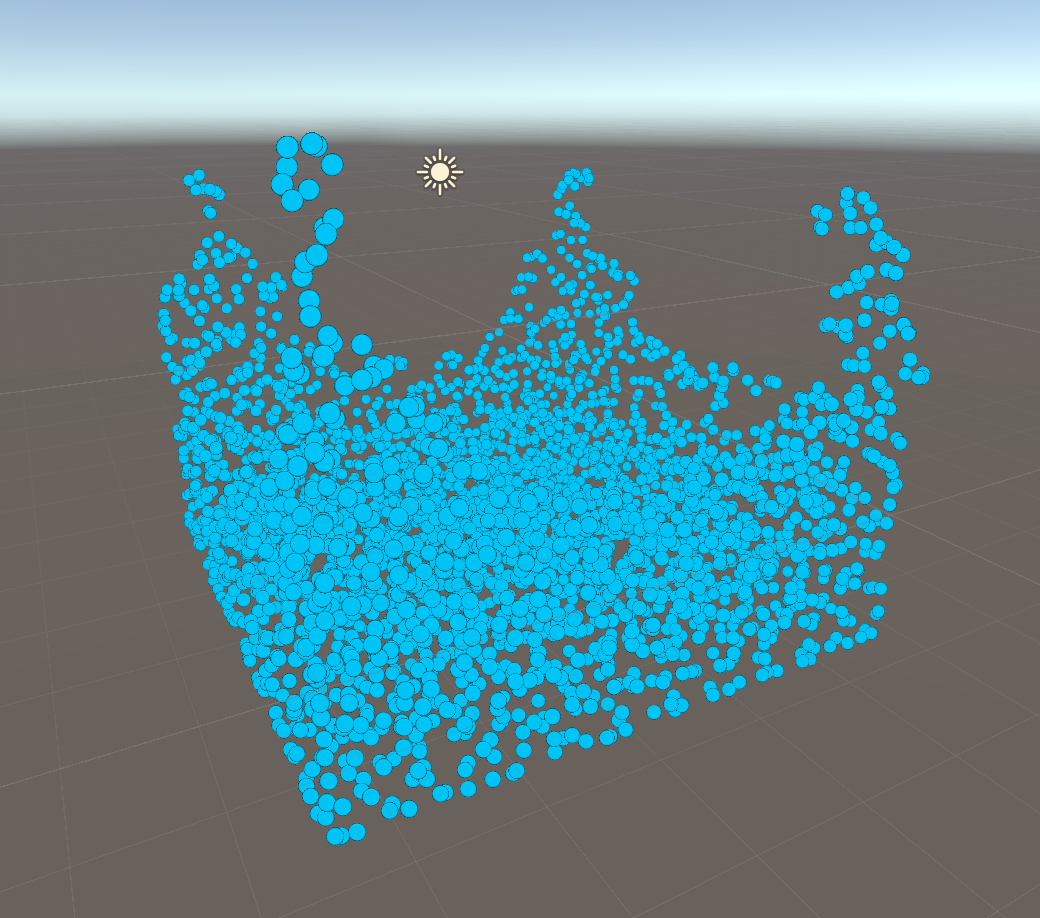
\includegraphics[width=0.9\linewidth]{../Images/Particles_Unity.PNG}
    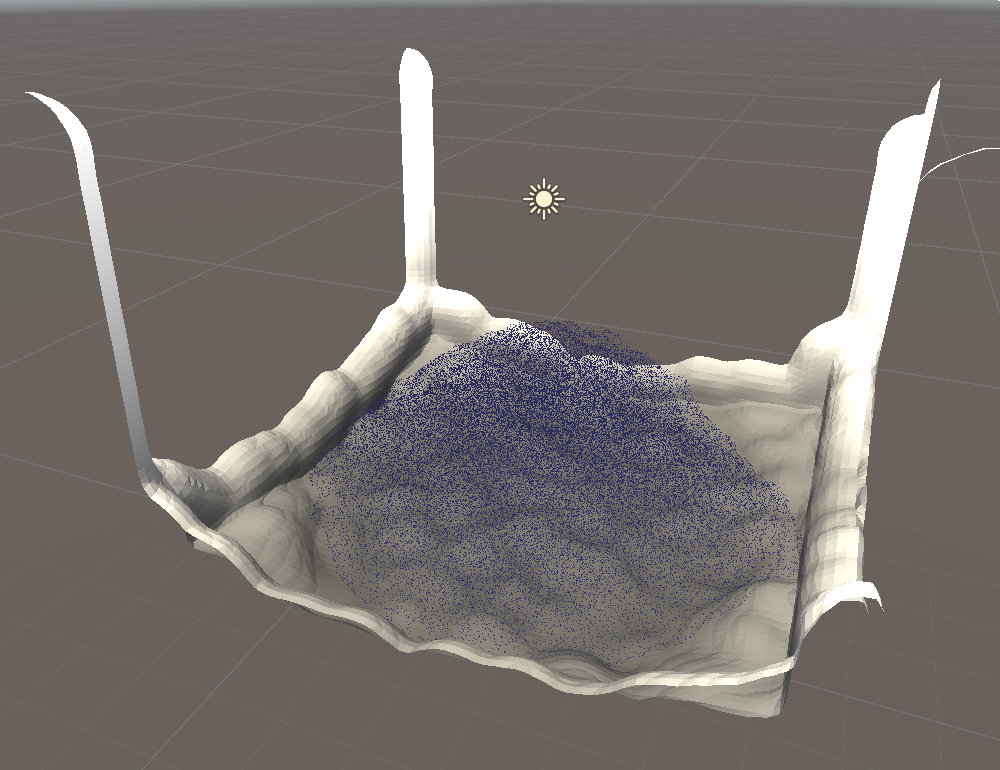
\includegraphics[width=0.9\linewidth]{../Images/Particles_GPU.PNG}
\end{center}

\subsection{Marching Cube}
Marching Cube can use to to many things related to CG.
In this project, we use marching cube to generate Meshes, directly render the volume matrix, 
and even use it to do the bounding coupling between solid volume matrix and fluid!.

1. Marching Cube Directly Rendering in shaderlab
Shaderlab with opengl(the wrap of hlsl of unity) can manually render various geometries using geometry shader. 
Inspired by this function, we in the end using the volume matrix data (only acces to the (x-1)*(y-1)*(z-1) points)
 as the start point of the triangle geometries of a voxel. In this situation, we do not need to record 
 a vertices list and a indices list to render the mesh, instead we directly map the volume matrix to the marching cube geometry.
 The following is an example of GPU rendered marching cube geometry:
 \begin{center}
     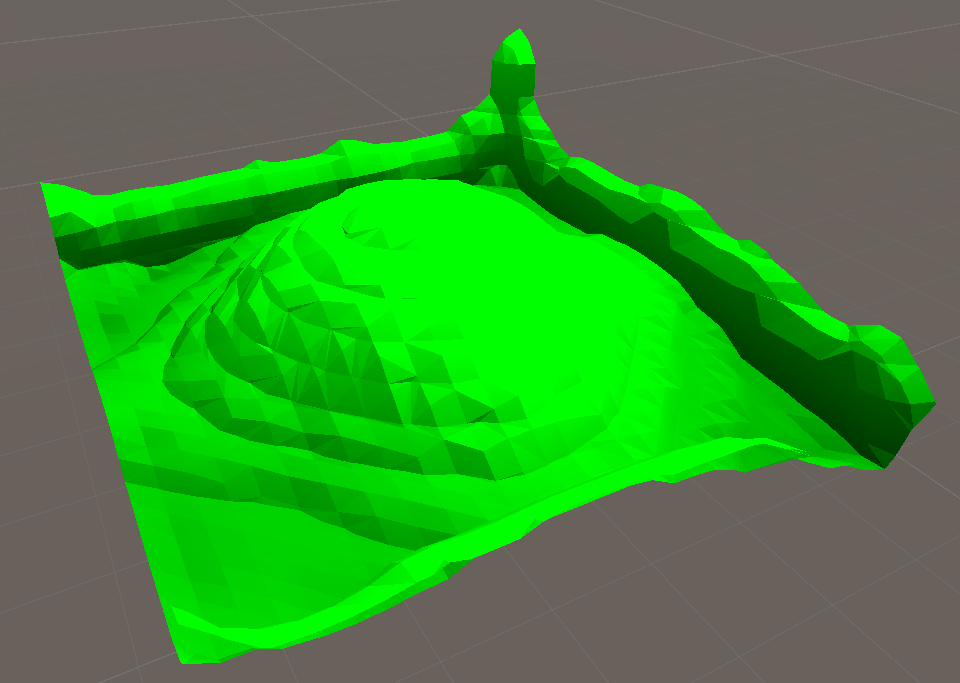
\includegraphics[width=0.9\linewidth]{../Images/MarchingCube_GPU.PNG}
 \end{center}


2. The marching cube technique is applied to generate the mesh and render according to the volume matrix. 
The whole process is divided into three passes. 
In the first pass, we traverse the voxel vertex data stored in the volume matrix 
to test whether its value is larger than the given isovalue and store the boolean result in another volume matrix. 
In the second pass, we traverse all edges of each voxel, the boolean value calculated in pass one can tell us 
whether there exists a vertex on this edge if the two boolean value are different. 
If so, we interpolate the two original value of voxel vertex to generate the vertex list. 
The result is stored in the vertex list. In the pass three, we traverse the voxel to generate the triangle, 
which can be enumerated into $2^8$ cases, but in fact one voxel can have at most 5 triangles. 
We store three index of each triangle into the index list. Then we can calculate the global coordinate 
of each triangle vertex according to index list and vertex list. 
Note that in pass two, a foreseeable better solution is to store both coordinate and global index together 
so that we do not need to know to each length of vertex index, as long as we use another array to store the bijection.
The followings are examples of CPU generated marching cube mesh:
\begin{center}
    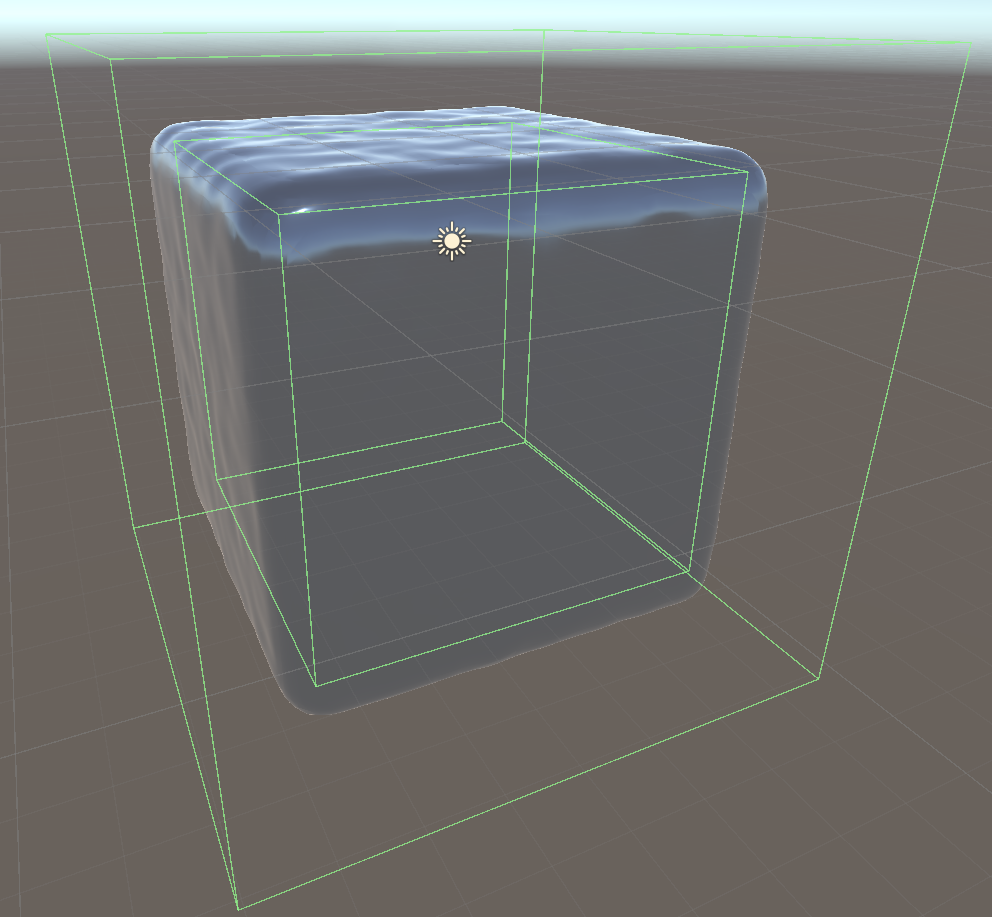
\includegraphics[width=0.9\linewidth]{../Images/MarchingCube_CPU_1.PNG}
    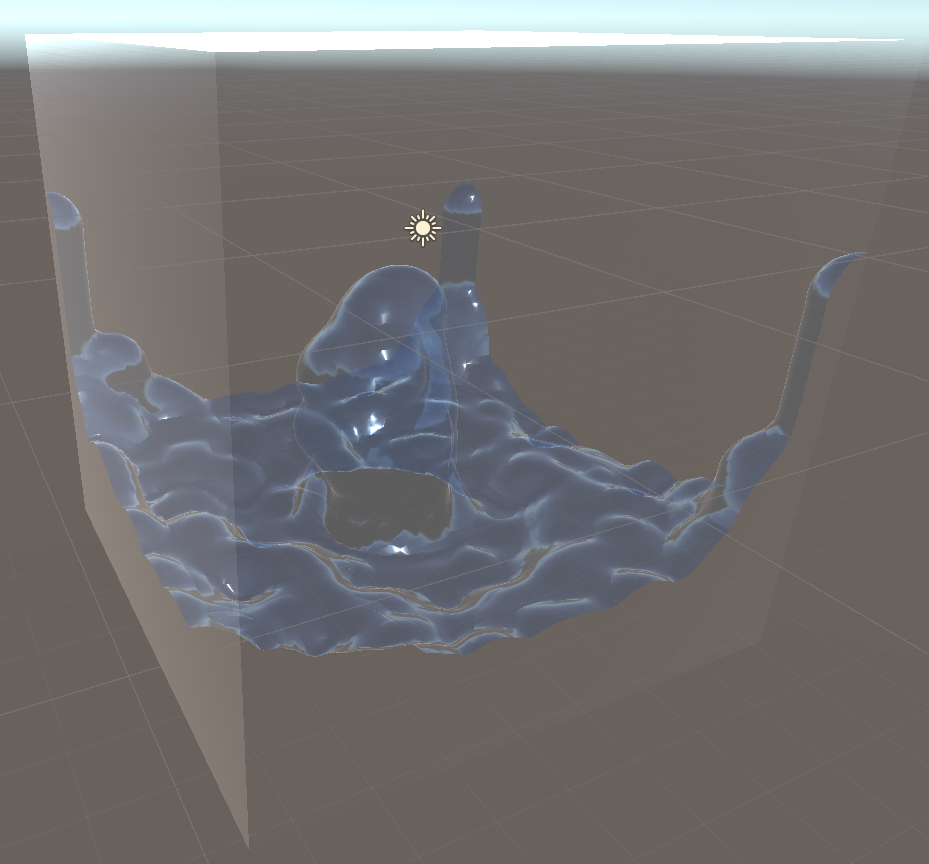
\includegraphics[width=0.9\linewidth]{../Images/MarchingCube_CPU_2.PNG}
\end{center}

\subsection{Conversion between Volume data And Particles}
We use a data structure to store volume data, which is called Volume Matrix.\\
The volume matrix store a $Vector3Int$ variable $size$ to record the size of the entire coordinate space, and a $float$ array $data$ to store the volulme value.\\
We also provides methods for storing a volume data to files and load volume data from files.\\
Volume data is commonly used in the whole simulation process. Rendering of the fluid surface, generating 3D terrain and fluid erosion all rely on volume data.\\
However, the PCISPH fluid simulator only simulates particle physics. Therefore, we need a converter to convert particle position data to volume data.\\
At the beginning, we implemented a algorithm that works by applying a blurring kernel to the volume data by each particle position (the kernel is needed to generate a continuous surface). This requires CPU to iterate over all particles, and for each particle iterate all volume points around it. GPU parallelization is not approachable since one volume point may affected by multiple particles at the same time.\\
After, we implemented an improved algorithm that uses the K-Nearest Neighbour algorithm (like in PCISPH) to find the neighbouring particles for each volume point, and accumulate the particles' contribution by the blurring kernel.\\
Although the new algorithm provides great performance enhancement, the conversion from particle to volume data is still costly. We may want to avoid this conversion to be executed every frame.

\subsection{Fluid-Solid Coupling Using Volume Data}
We implemented a fluid-solid coupling algorithm using volume data for each particle. \\
The advantage of the algorithm is the coupling operation can be done individually by one particle with the volume grid the particle in. Thus we do not need to traverse all surfaces in the scene (or use a acceleration structure), and the algorithm is fully parallelized in GPU, integrated in the PCISPH compute shader.\\
Each time we need to detect collision for a particle, we get the volume grid the particle is in by its posisiton, use the Marching Cube technique to find the possible triangles in the grid, and use the ray-single-triangle-intersection method to detect whether a collision has taken place.\\
As long as one collision is found, the velocity and position of the particle is corrected in the reflection direction.
The following is an example of fluid-solid coupling with terrain:
\begin{center}
    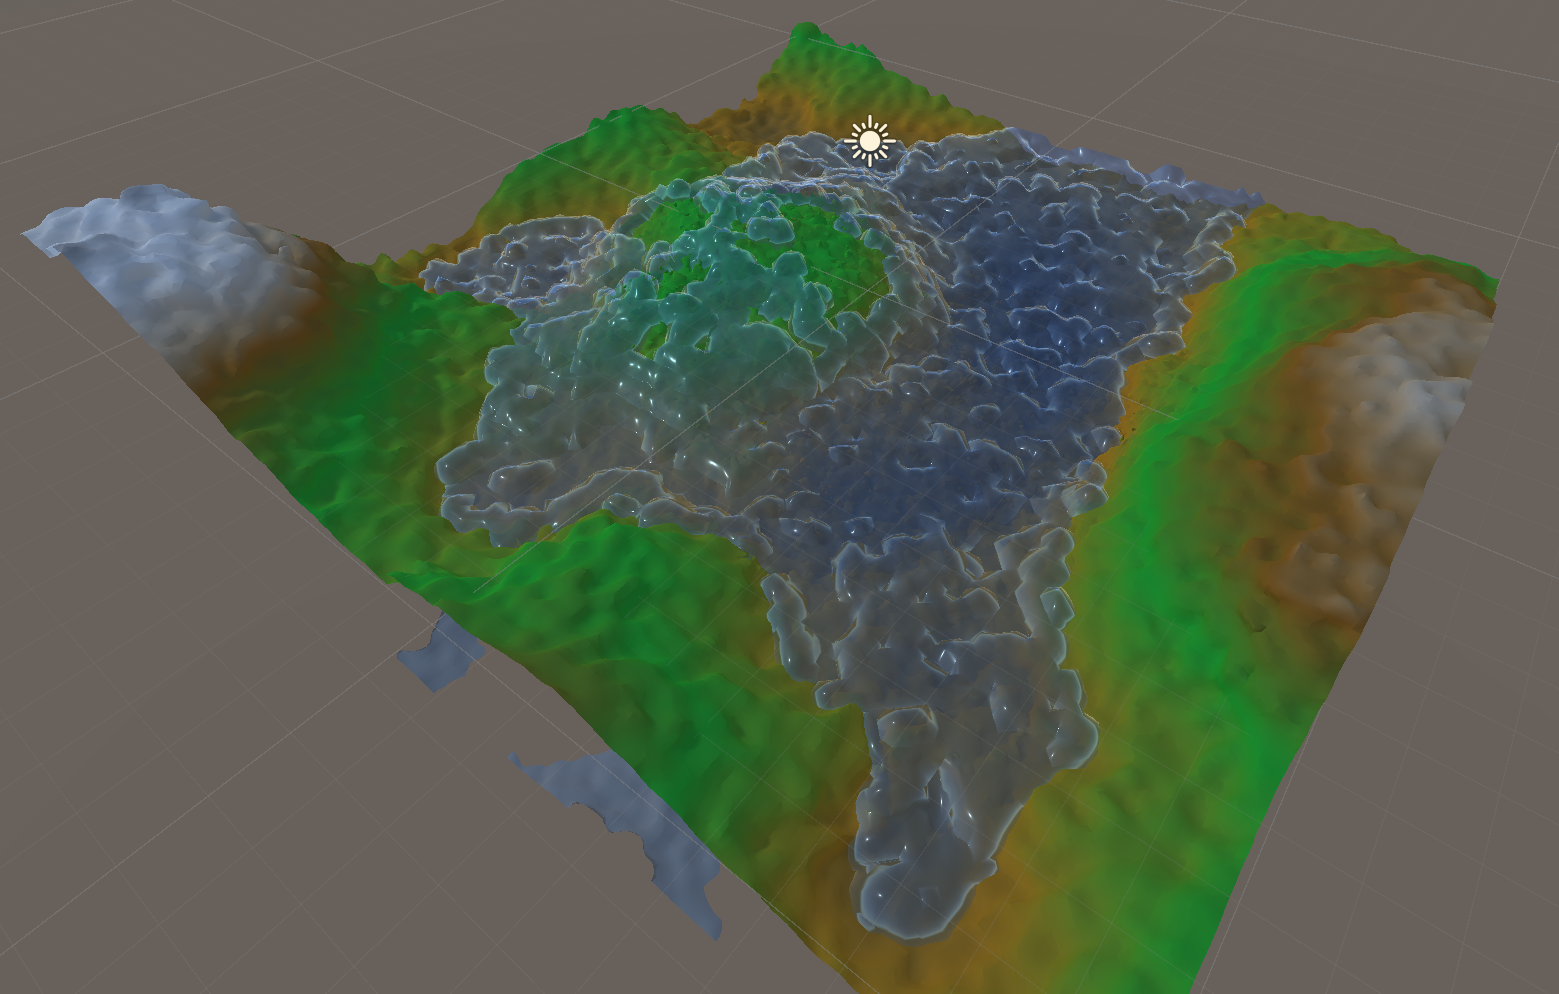
\includegraphics[width=0.9\linewidth]{../Images/Coupling.PNG};
\end{center}

\subsection{Terrain Generation With Noise}
We apply 3 dimensional Perlin Noise to generate a volume data at each spatial coordinate in the bounding box we set.
It is naturally that we package the volume data into the volume matrix in the purpose of building the terrain.
In practice, we use noise layers to generate different terrain by changing the weight of each layer in the entire part.
We also set parameters $sharpness$ and $magnitude$ to restrain the spatial distribution of the terrain. \\
We generate the perlin noise of each spatial coordinate in the computer shader at differrent threads, which runs on the GPU. This can enable real-time terrain re-generation, which greatly helps creators to generate desired terrain.\\

\subsection{Terrain Coloring}
We designed a color curve to approximately simulate the surface appearance of real terrain.
The color is mapped according to the height and normal direction.
In general, the larger the height and the closer the normal direction with the positive y-axis direciton,
the larger the value will be in the color curve. As a result, we can generate a terrian with river valley,
meadow in the midium to height altitude and the ice sheet on the peak.\\
The following is an example of generated terrain:\\
\begin{center}
    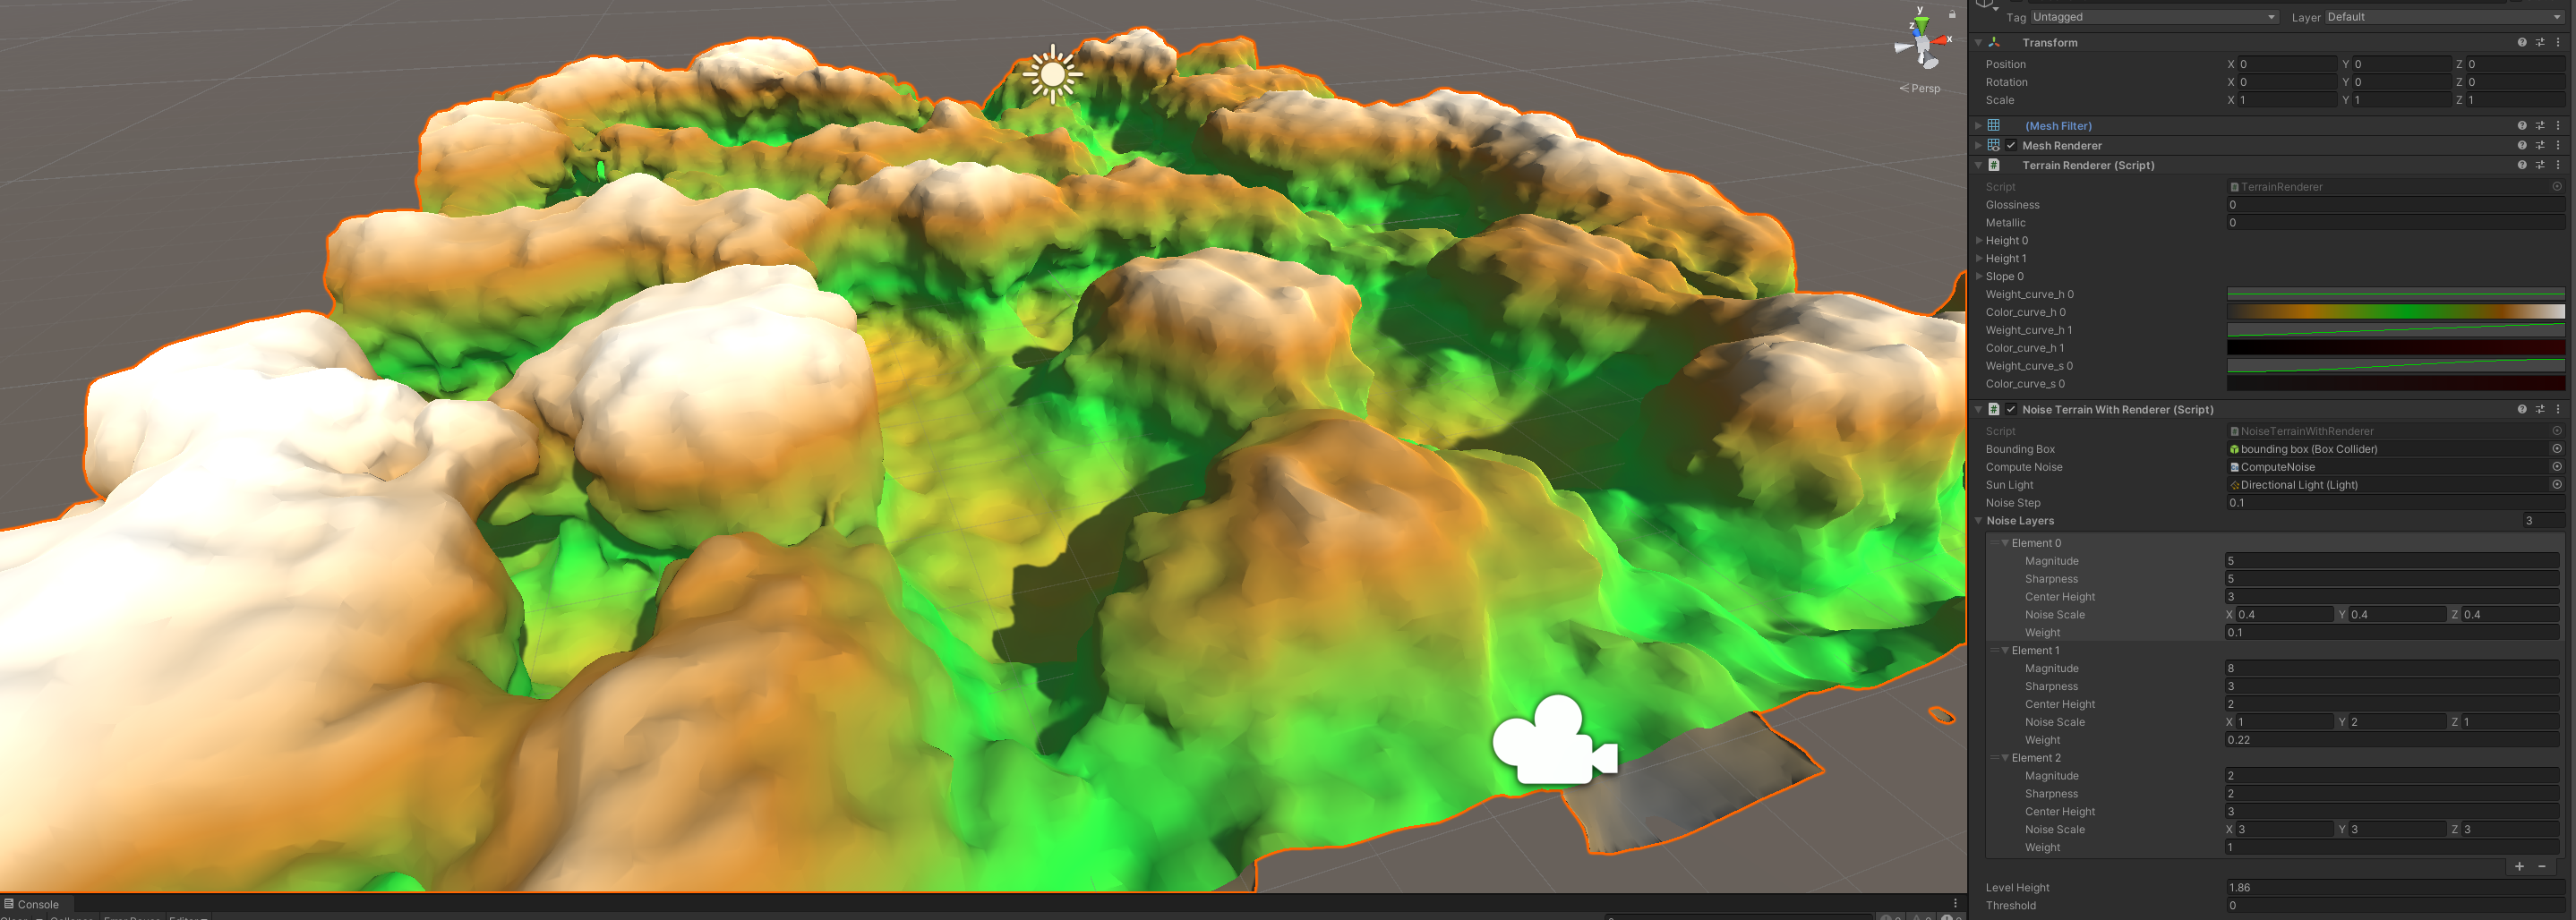
\includegraphics[width=0.9\linewidth]{../Images/NoiseTerrain.PNG}
\end{center}

\subsection{Terrain (Volume Data) Erosion}
We developed a terrain erosion algorithm based on the previous fluid-solid coupling algorithm. The erosion can apply to any volume data.\\
In the detection of collision between fluid particle and the terrain (volume data), if one collision is detected, the GPU saves the collision info, including the collision position, collision normal and particle momentum.\\
When all the collisions are calculated, the CPU handles the erosion process itself. It iterates all collisions, calculate the erosion based on the collision info.\\
The following is the corresponding erosion result of the previous example of fluid-solid coupling:\\
\begin{center}
    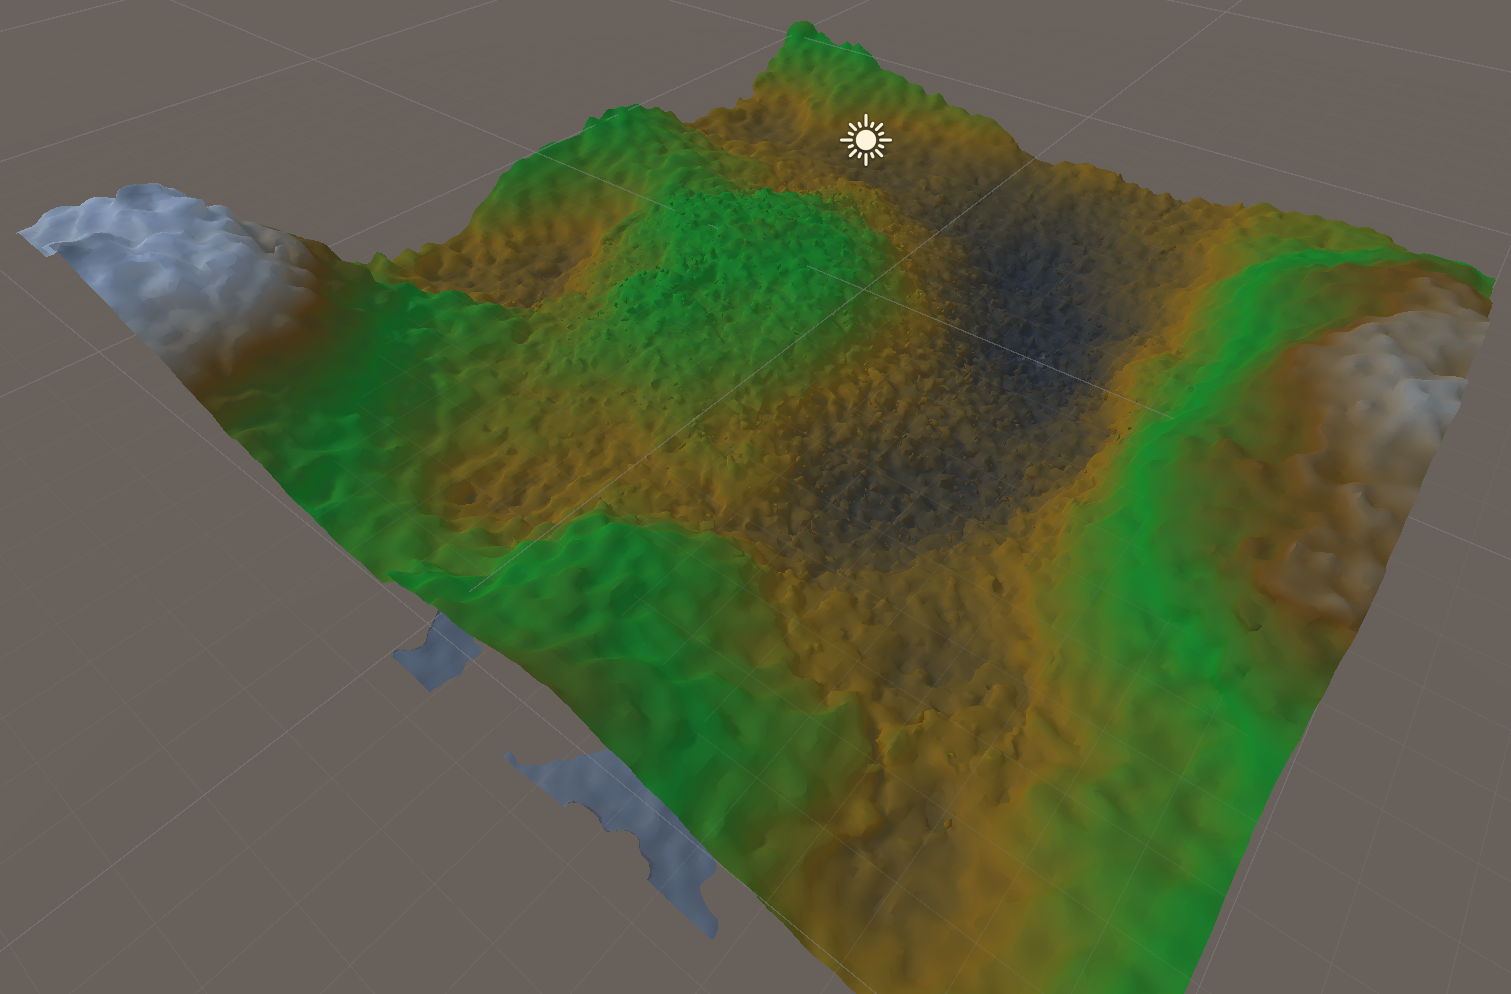
\includegraphics[width=0.9\linewidth]{../Images/Coupling_Erosion}
\end{center}
Here is the same terrain before and after multiple iterations of erosion process:
\begin{center}
    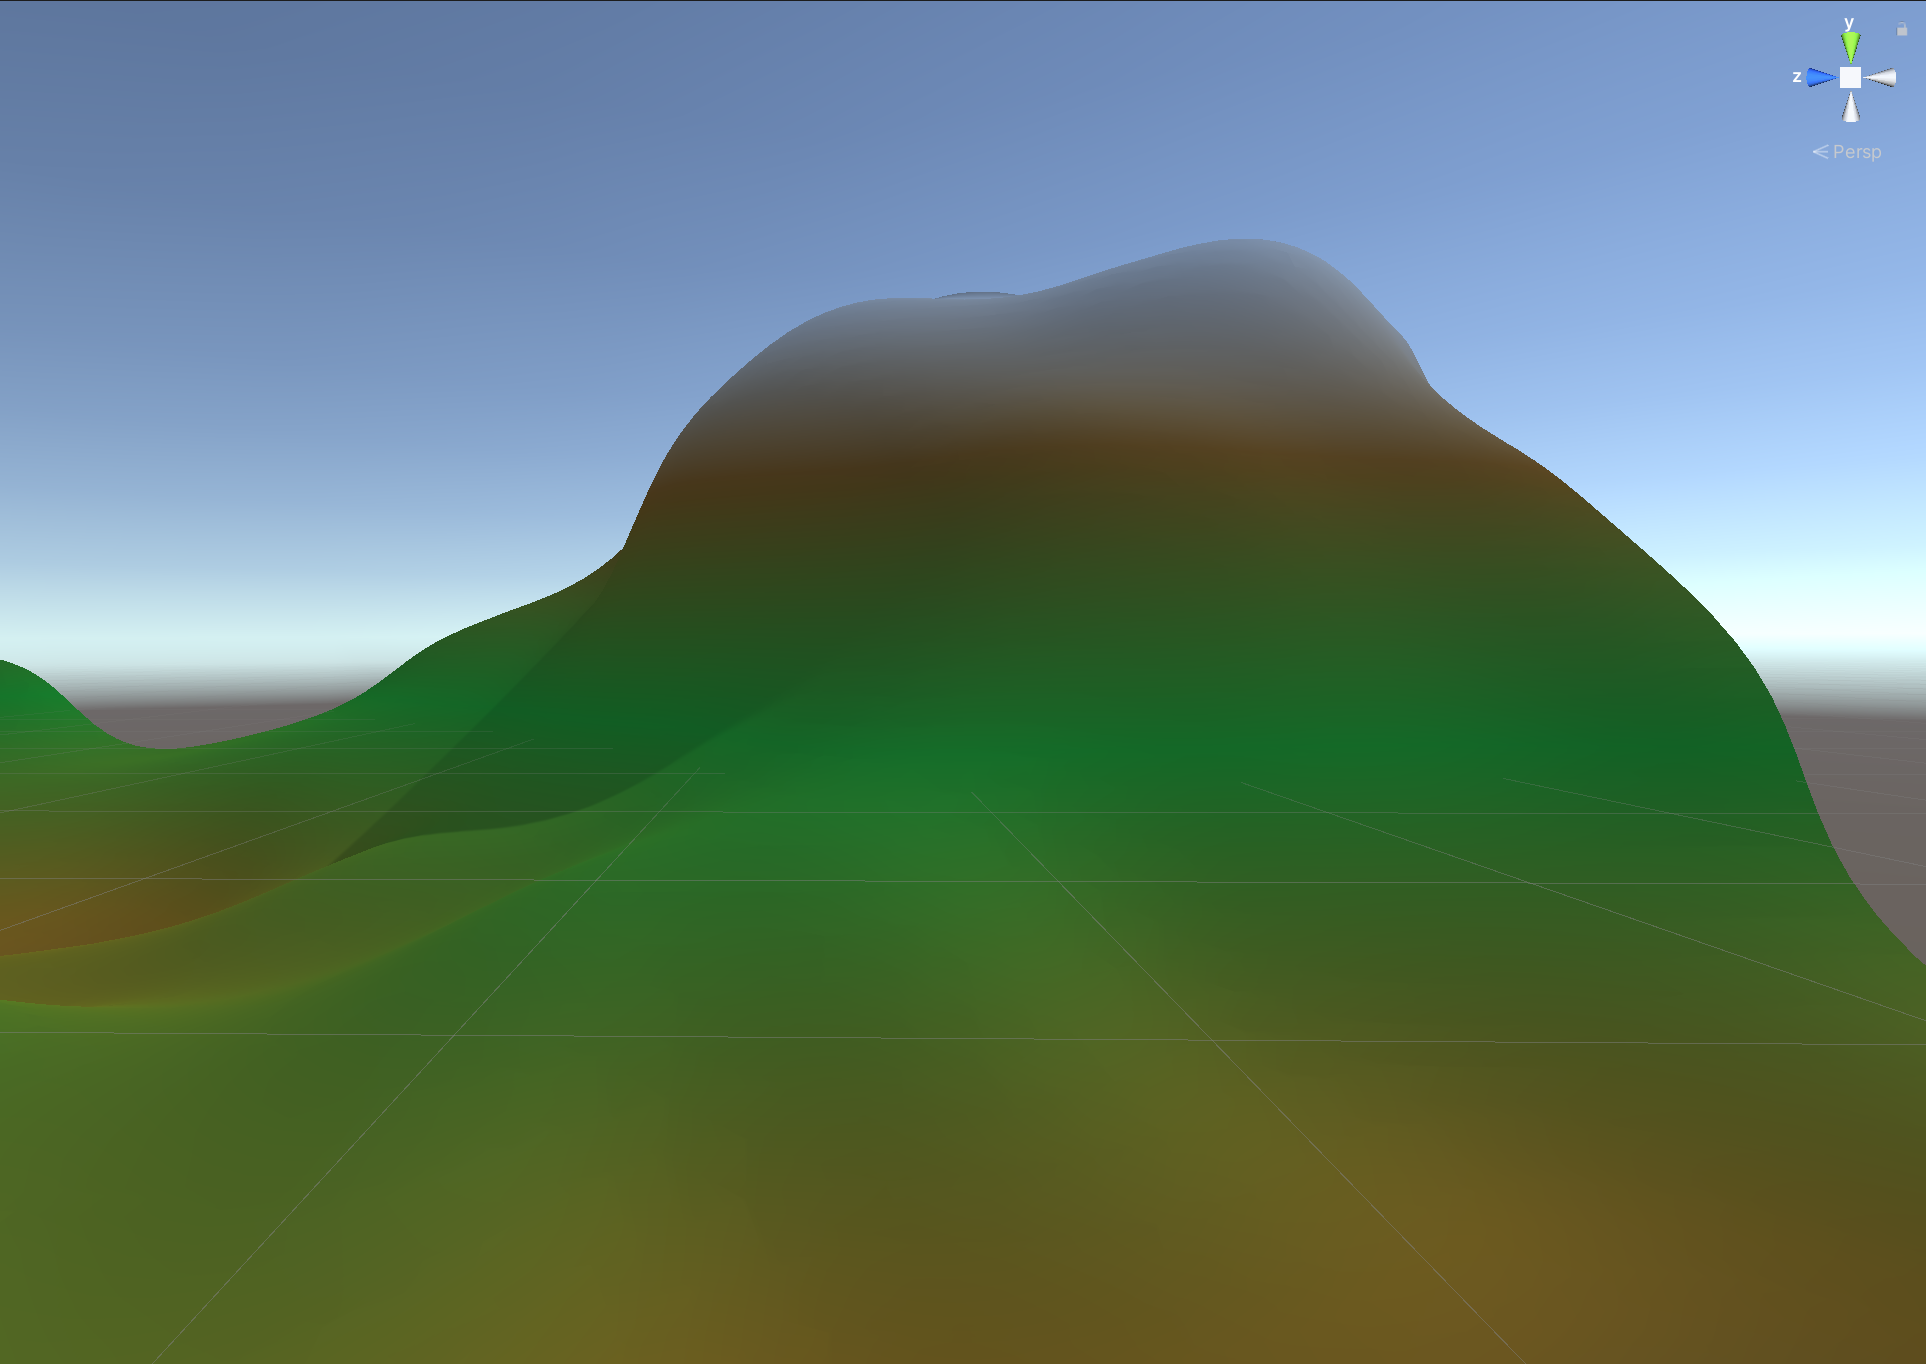
\includegraphics[width=0.9\linewidth]{../Images/Erosion_Before.png}
    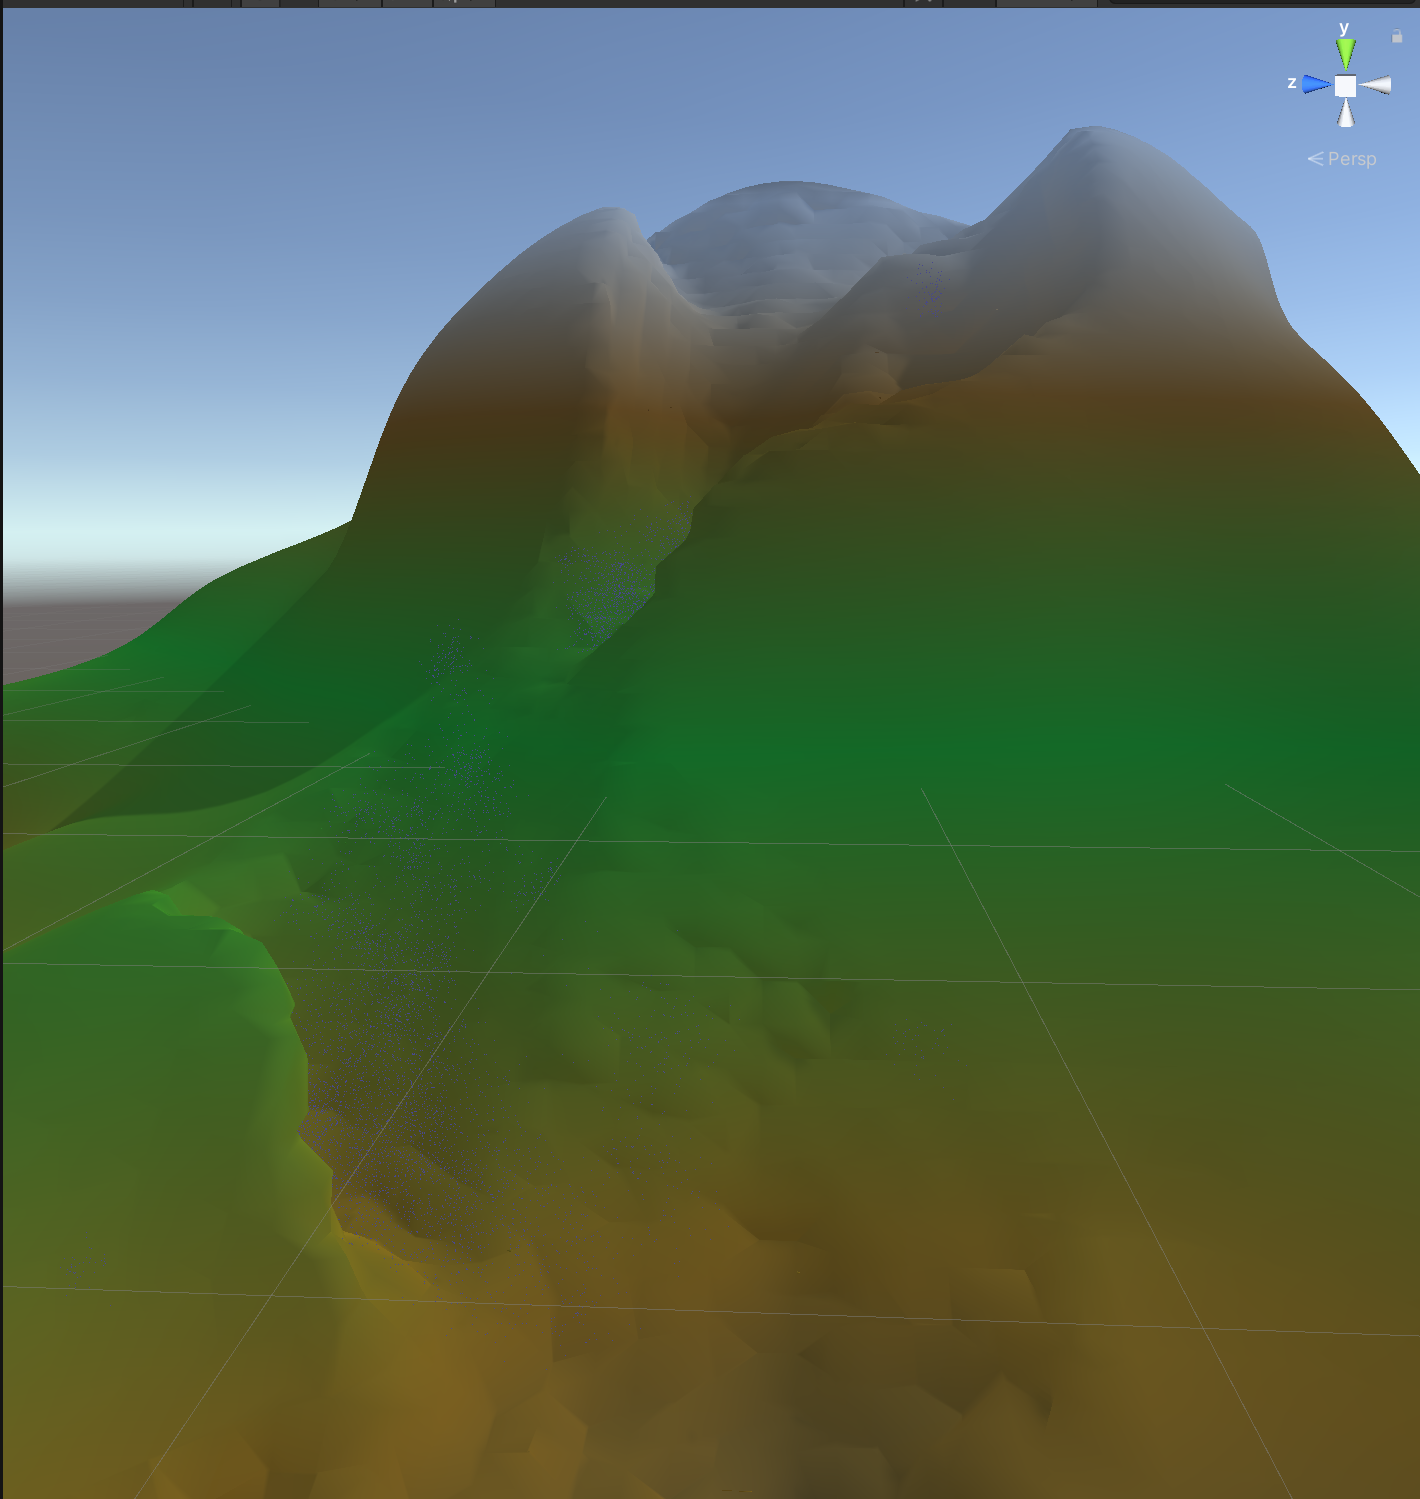
\includegraphics[width=0.9\linewidth]{../Images/Erosion_After.png}
\end{center}

\section{Results}
Here are some examples of beautiful realistic terrains generated by multiple scale Perlin noises and marching cube:
\begin{center}
    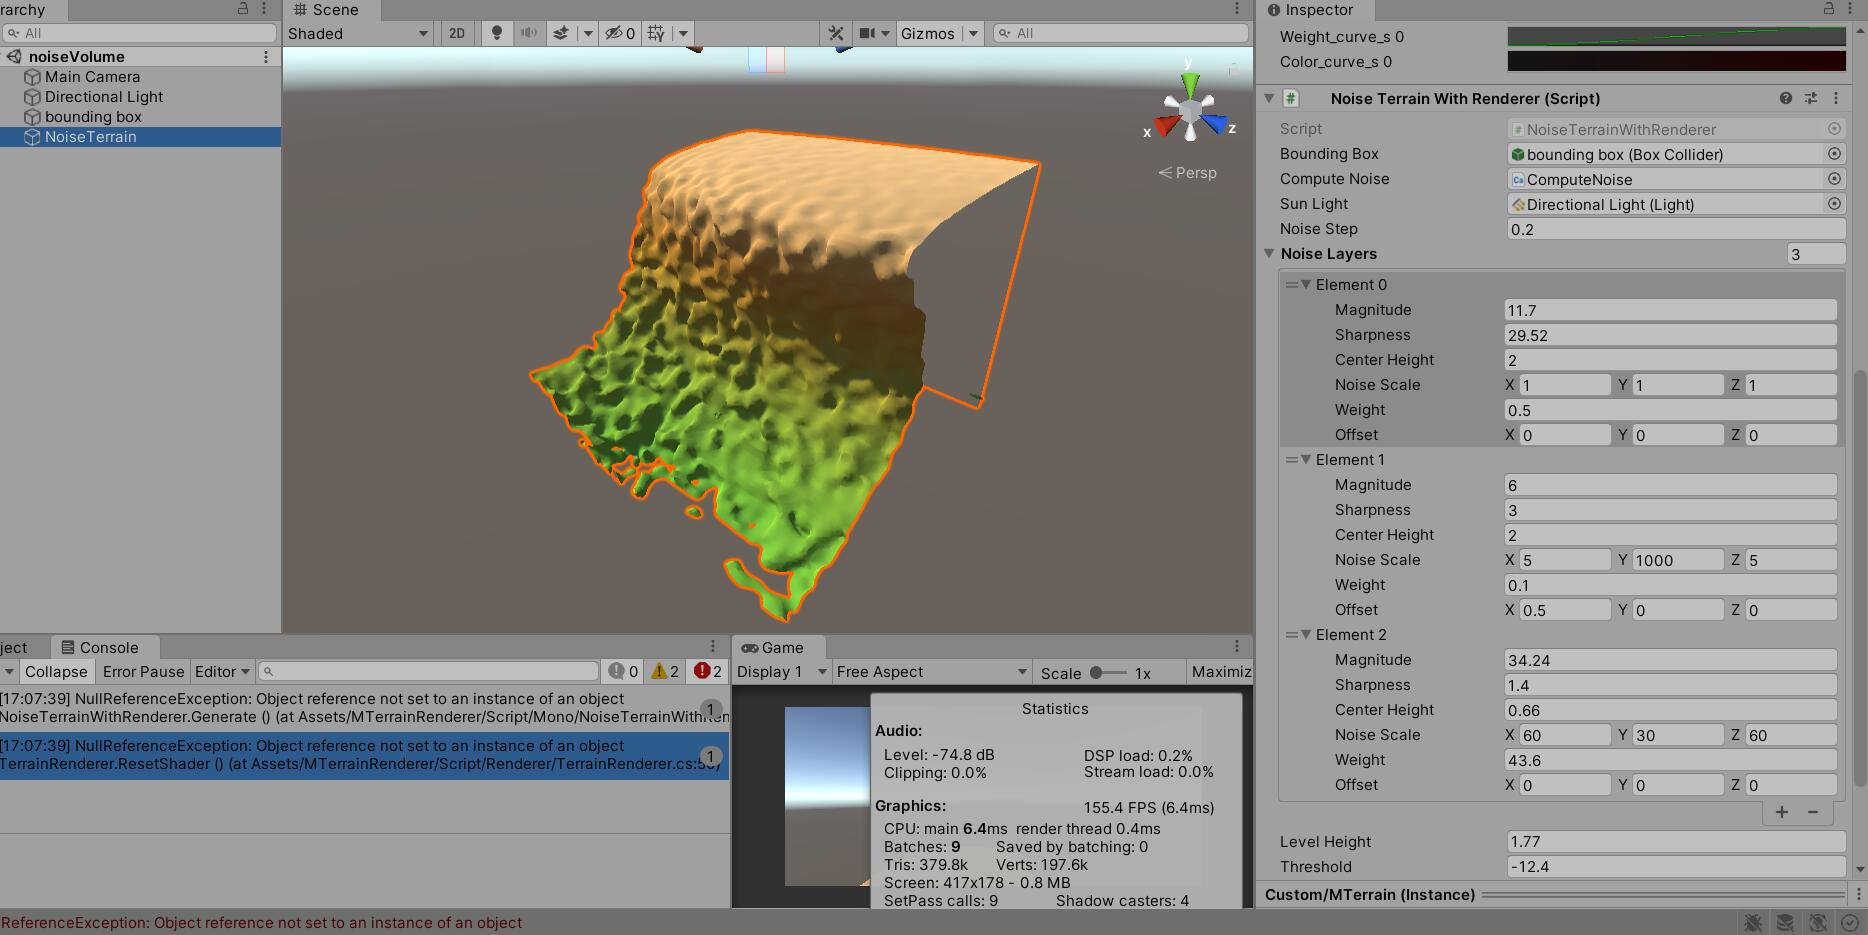
\includegraphics[width=0.9\linewidth]{../Images/Terrain_0.jpg}
    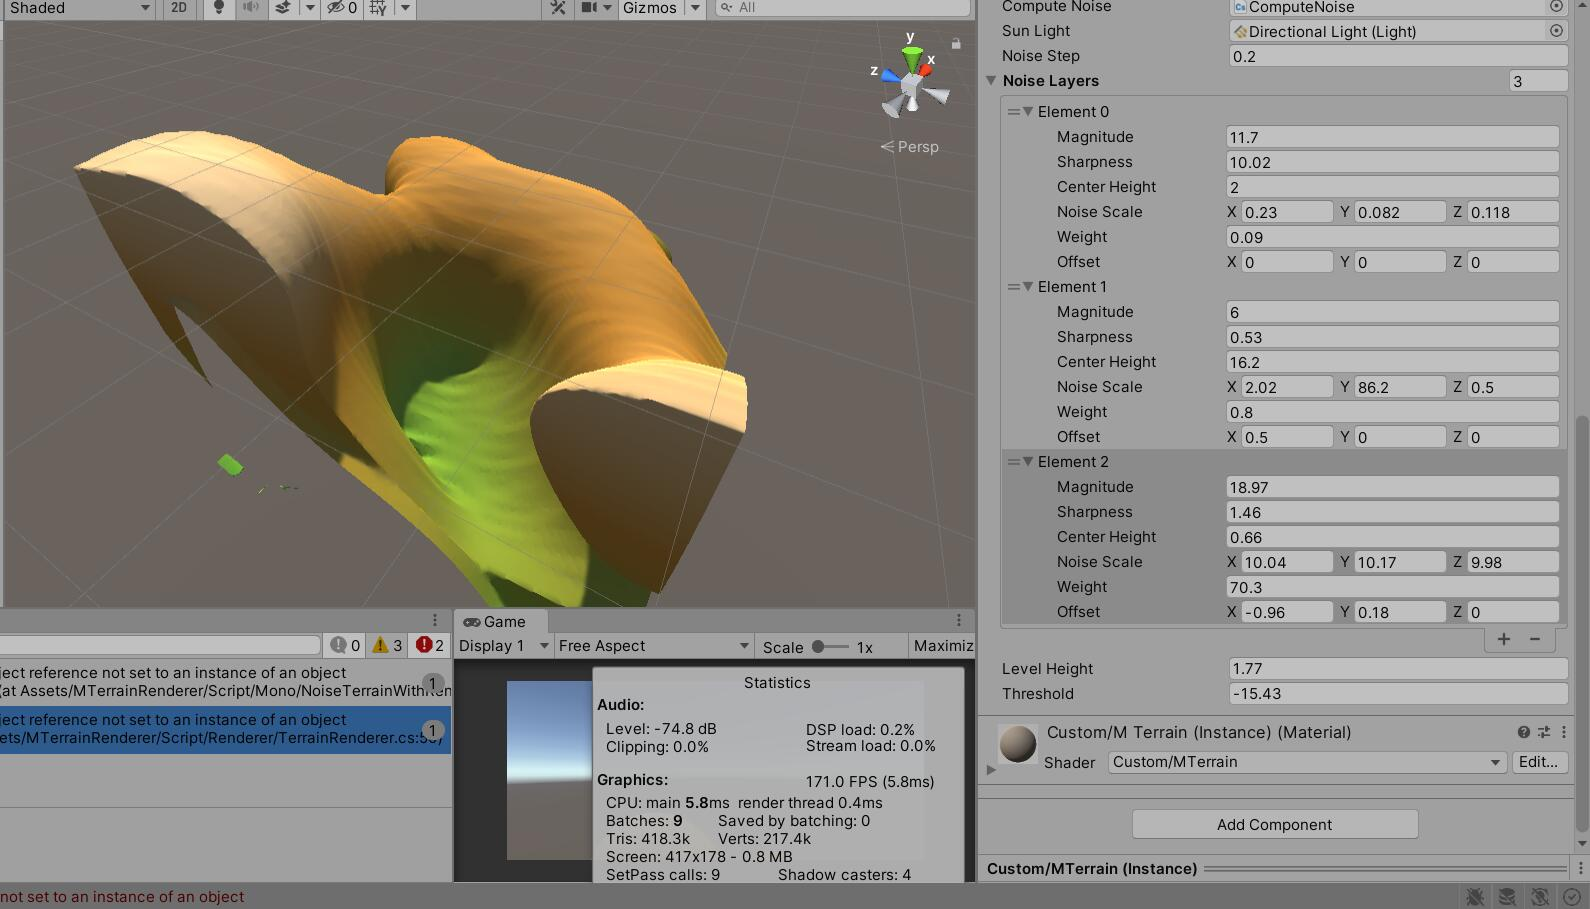
\includegraphics[width=0.9\linewidth]{../Images/Terrain_1.jpg}
\end{center}

\section{Conclusion}
We give a unique method of terrain generation using Perlin noise and physically based fluid erosion.\\
With the support of Unity editor, creators can customize their preferred terrain and export for further uses.

\end{document}
